\حصہ{فشار سیال اور قوت سیال}
فشار \عددی{p} سے مراد وہ قوت ہے جو اکائی رقبہ پر عمل کرتی ہو۔ یوں اگر رقبہ \عددی{S} پر قوت \عددی{F} عمل کرتی ہو تب فشار \عددی{p} درج ذیل ہو گا۔
\begin{align}\label{مساوات_تکمل_استعمال_فشار_اور_قوت}
p=\frac{F}{S}
\end{align}
\جزوحصہء{مستقل گہرائی پر قوت سیال اور فشار سیال}
 شکل \حوالہ{شکل_تکمل_استعمال_فشار_سیال_تعریف} میں ساکن سیال کو ایک برتن میں دکھایا گیا ہے جہاں تلا کا رقبہ \عددی{S}، سیال کی گہرائی \عددی{h} اور  سیال کی کثافت \عددی{\rho} ہے۔ یوں سیال کا حجم \عددی{Sh}،  کمیت \عددی{\rho Sh} اور وزن \عددی{g\rho Sh} ہو گا۔ سیال کے وزن کے برابر قوت \عددی{F=g\rho Sh} رقبہ \عددی{S} پر عمل کرے گی۔ یوں اکائی رقبہ پر قوت \عددی{g\rho h} ہو گی جس کو \اصطلاح{فشار}\فرہنگ{فشار}\حاشیہب{pressure}\فرہنگ{pressure} \عددی{p} یا \اصطلاح{دباو}\فرہنگ{دباو}  کہتے ہیں۔
\begin{align}\label{مساوات_تکمل_استعمال_فشار_سیال_الف}
p&=\rho g h
\end{align}
فشار کی اکائی  نیوٹن فی مربع میٹر \عددی{\si{\newton\per\meter\squared}} ہے۔ آپ نے دیکھا کہ سیال کی قیمت پر برتن کی صورت کا کوئی اثر نہیں پایا جاتا ہے۔

 مستقل گہرائی کے رقبہ \عددی{S} پر درج ذیل قوت پائی جائے گی۔
\begin{align}
F=pS
\end{align}
%
\begin{figure}
\centering
\begin{minipage}{0.45\textwidth}
\centering
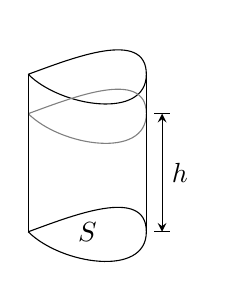
\begin{tikzpicture}[]
\pgfmathsetmacro{\h}{2}
\pgfmathsetmacro{\r}{1.5}
\draw(0,0)to [out=-45,in=-90] ++(\r,0) to [out=90,in=20]++(-\r,0);
\draw(0,\h)to [out=-45,in=-90] ++(\r,0) to [out=90,in=20]++(-\r,0);
\draw[gray](0,3/4*\h)to [out=-45,in=-90] ++(\r,0) to [out=90,in=20]++(-\r,0);
\draw(0,0)--++(0,\h)  (\r,0)--++(0,\h);
\draw(\r+0.1,0)--++(0.2,0)coordinate[pos=0.5](k);
\draw(\r+0.1,3/4*\h)--++(0.2,0);
\draw[stealth-stealth](k)--++(0,3/4*\h)node[pos=0.5,right]{$h$};
\draw(0.75,0)node[]{$S$};
\end{tikzpicture}
\caption{فشار سیال۔}
\label{شکل_تکمل_استعمال_فشار_سیال_تعریف}
\end{minipage}\hfill
\begin{minipage}{0.45\textwidth}
\centering
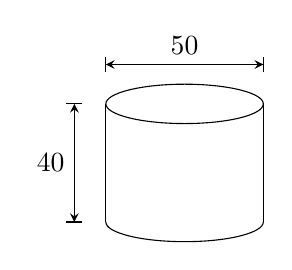
\begin{tikzpicture}
\pgfmathsetmacro{\h}{1.5}
\pgfmathsetmacro{\r}{1}
\draw([shift={(180:\r cm and 1/4*\r cm)}]0,0) arc (180:360:\r cm and 1/4*\r cm);
\draw(0,\h) circle (\r cm and 1/4*\r cm);
\draw(-\r,0)--++(0,\h)  (\r,0)--++(0,\h);
\draw[stealth-stealth](-\r,\h+0.5)--++(2*\r,0)node[pos=0.5,above]{$\SI{50}{\meter}$};
\draw(-\r,\h+0.4)--++(0,0.2)  (\r,\h+0.4)--++(0,0.2);
\draw[stealth-stealth](-\r-0.4,0)--++(0,\h)node[pos=0.5,left]{$\SI{40}{\meter}$};
\draw(-\r-0.3,0)--++(-0.2,0)  (-\r-0.3,\h)--++(-0.2,0);
\end{tikzpicture}
\caption{بیلنی حوض برائے مثال \حوالہ{مثال_تکمل_استعمال_بیلنی_حوض_نچلی_پٹی}}
\label{شکل_مثال_تکمل_استعمال_بیلنی_حوض_نچلی_پٹی}
\end{minipage}
\end{figure}

سیال میں \عددی{h} گہرائی پر کسی بھی رخ فشار کی قیمت  مساوات \حوالہ{مساوات_تکمل_استعمال_فشار_سیال_الف} دیتی ہے۔ یوں کسی بھی گہرائی پر افقی اور انتصابی دیواروں پر فشار کی قیمت ایک دوسرے جیسی ہو گی۔ 

\ابتدا{مثال}\شناخت{مثال_تکمل_استعمال_بیلنی_حوض_نچلی_پٹی}
ایک بیلنی حوض میں پانی کی گہرائی  \عددی{\SI{40}{\meter}} ہے  جبکہ حوض کا رداس \عددی{\SI{25}{\meter}} ہے (شکل \حوالہ{شکل_مثال_تکمل_استعمال_بیلنی_حوض_نچلی_پٹی})۔ حوض کے اطراف کی دیوار کی نچلی \عددی{\SI{1}{\meter}}  پٹی  پر فشار سیال اور قوت سیال کتنا ہو گا؟ (پانی کی کثافت کو \عددی{\rho=\SI{1000}{\kilo\gram\per\meter\cubed}} لیں۔)

حل: \quad
 اس ایک میٹر چوڑی پٹی کے  نچلے کنارے پر فشار درج ذیل ہو گا۔
\begin{align*}
p=\rho g h=(1000)(9.8)(40)=\SI{392000}{\newton\per\meter\squared}
\end{align*}
ایک میٹر پٹی کا رقبہ
\begin{align*}
S=2\pi r h=2\pi(25)(1)=50\pi\,\si{\meter\squared}
\end{align*}
ہے لہٰذا اس پر کل قوت درج ذیل ہو گی۔
\begin{align*}
F=pS=(392000)(50\pi)=\SI{61575216.01}{\newton}
\end{align*}
\انتہا{مثال}
%====================

اس مثال میں پٹی کے نچلے حصے کی گہرائی \عددی{\SI{40}{\meter}} اور بالائی حصے کی گہرائی \عددی{\SI{39}{\meter}} تھی  لہٰذا ان پر فشار پر مختلف ہو گا۔ ہم نے اس حقیقت کو نظر انداز کیا۔ آئیں متغیر گہرائی کی صورت میں فشار پر غور کریں۔

\جزوحصہء{متغیر گہرائی پر فشار}
فرض کریں ہم کثافت \عددی{\rho} کی سیال میں ڈوبے ہوئے انتصابی تختی کی ایک طرف پر قوت سیال جاننا چاہتے ہیں۔ ہم تختی کو \عددی{xy} مستوی میں خطہ \عددی{y=a} تا \عددی{y=b} تصور کرتے ہیں (شکل \حوالہ{شکل_تکمل_استعمال_قوت_سیال})۔ ہم \عددی{[a,b]} کی خانہ بندی کرتے ہیں۔ ہم اس خطہ کو نقاط خانہ بندی پر محور \عددی{y} کے عمودی فرضی سطحوں سے باریک افقی پٹیوں میں تقسیم کرتے ہیں۔ ایک نمائندہ پٹی جو \عددی{y} سے \عددی{y+\Delta y} تک ہو کی چوڑائی \عددی{\Delta y} ہو گی جبکہ اس پٹی کے نچلی ضلع کی لمبائی \عددی{L(y)} ہو گی۔ ہم فرض کرتے ہیں کہ \عددی{L(y)} متغیر \عددی{y} کا استمراری تفاعل ہے۔
\begin{figure}
\centering
\begin{tikzpicture}[font=\small]
\draw[-latex](-0.5,-0.2)--++(0,2.5)node[above]{$y$};
\draw[name path=fluid,thick](-0.75,1.75)--(5.5,1.75)node[right,]{\RL{سطح سیال}};
\draw[name path=fun] plot [smooth cycle]coordinates {(0,0.75)(0.5,0.25)(1.5,0)(3.5,0.25)(4,0.75)(3.5,1)(2.5,0.75)(0.5,1.25)};
\draw[dashed](0.5,1.25)--(-0.5,1.25)node[left]{$b$};
\draw[dashed](1.5,0)--(-0.5,0)node[left]{$a$};
\path[name path=lineA](-0.2,0.4)--++(4.2,0);
\path[name path=lineB](-0.2,0.4+0.1)--++(4.2,0);
\draw[name intersections={of=fun and lineA, by={kka,kkb}}](kka)--(kkb);
\draw(kka)++(0.05,-0.1)--++(0,-0.75)coordinate[pos=0.8](a);
\draw(kkb)++(-0.05,-0.1)--++(0,-0.75)coordinate[pos=0.8](b);
\draw[stealth-stealth](a)--(b)node[pos=0.5,below]{$L(y)$};
\draw(kka)++(0.2,0)--++(0.75,0)coordinate[](kk)coordinate[pos=0.9](c)coordinate[pos=0.5](kL);
\draw(kk)++(0,0.1)--++(-0.2,0);
\draw[stealth-](c)--++(0,-0.2);
\draw[stealth-](c)++(0,0.1)--++(0,0.2)--++(0.2,0)node[right]{$\Delta y$};
\draw[stealth-stealth](kL)--($(0,1.75)!(kL)!(4,1.75)$)node[pos=0.65,fill=white]{\RL{گہرائی پٹی}};
\draw[dashed](kka)++(-0.1,0)--($(-0.5,0)!(kka)!(-0.5,1)$)node[left]{$y$};
\draw[name intersections={of=fun and lineB,by={kkc,kkd}}](kkc)--(kkd);
\fill[lgray](kka)--(kkb)--(kkd)--(kkc)--(kka);
\draw(2.5,0.75)--++(-0.5,0.4)node[above]{\RL{سیال میں ڈوبی انتصابی تختی}};
\end{tikzpicture}
\caption{ایک پتلی پٹی پر قوت سیال۔}
\label{شکل_تکمل_استعمال_قوت_سیال}
\end{figure}

نیچے سے اوپر چلتے ہوئے گہرائی کی تبدیلی سے پٹی پر فشار تبدیل ہوتا ہے۔ اب اگر پٹی کی چوڑائی بہت کم ہو تب فشار کی اس تبدیلی کو رد کیا جا سکتا ہے اور ہم کہہ سکتے ہیں کہ پٹی پر ہر جگہ فشار وہی ہو گا جو پٹی کی نچلی کنارے پر ہے۔ یوں پٹی کی ایک طرف پر قوت درج ذیل ہو گی۔
\begin{align*}
\Delta F&=(\text{\RL{پٹی کے نچلے کنارے پر فشار}})(\text{\RL{رقبہ پٹی}})\\
&=\rho g (\text{\RL{گہرائی پٹی}})L(y)\Delta y
\end{align*} 
پورے تختی پر قوت تخمیناً 
\begin{align}
\sum_a^b \Delta F=\sum_a^b \rho g (\text{\RL{گہرائی پٹی}})L(y)\Delta y
\end{align}
ہو گی جو \عددی{[a,b]} پر استمراری تفاعل کا ریمان مجموعہ ہے۔ ہم توقع کرتے ہیں کہ خانہ بندی کا معیار صفر تک پہنچنے سے یہ مجموعہ بہتر سے بہتر نتیجہ دے گا۔ ہم ان مجموعوں کی تحدیدی قیمت کو  تختی پر قوت کی تعریف لیتے ہیں۔

\ابتدا{تعریف}\موٹا{تکمل برائے قوت سیال}\\
فرض کریں محور \عددی{y} پر \عددی{y=a} سے \عددی{y=b} تک کا خطہ، سیال میں ڈوبے ہوئی ایک تختی کو ظاہر کرتا ہے۔مزید فرض کریں کہ \عددی{y} پر اس تختی کی سطح پر افقی پٹی  کی بائیں سے دائیں  لمبائی \عددی{L(y)} ہے۔ اس تختی کی ایک طرف پر قوت سیال درج ذیل ہو گا۔
\begin{align}
F=\int_a^b\rho g \cdot(\text{\RL{گہرائی پٹی}})\cdot L(y)\dif y
\end{align}
\انتہا{تعریف}
%=================

\ابتدا{مثال}\شناخت{مثال_تکمل_استعمال_مثلث_قوت_پانی}
ایک مساوی الساقین مثلث تختی جس کا تلا \عددی{\SI{4}{\meter}} اور قد \عددی{\SI{2}{\meter}} ہے ایک پانی کے تالاب میں یوں ڈوبا ہوا ہے کہ اس کا تلا اوپر ہو۔ تلا پر پانی کی گہرائی \عددی{\SI{1.5}{\meter}} ہے۔ تختی کے ایک طرف پر قوت تلاش کریں۔ (پانی کی کثافت کو \عددی{\rho=\SI{1000}{\kilo\gram\per\meter\cubed}} لیں۔)

حل:\quad
ہم تختی کی نچلی راس کو محدد کے مبدا پر تصور کرتے ہیں (شکل \حوالہ{شکل_مثال_تکمل_استعمال_مثلث_قوت_پانی})۔یوں سطح پانی \عددی{y=3.5} پر ہو گا جبکہ تختی کا بالائی کنارہ \عددی{y=2} پر ہو گا۔تختی کا دایاں کنارہ \عددی{y=x} اور بایاں کنارہ \عددی{y=-x} ہو گا۔ یوں \عددی{y} پر پٹی کی لمبائی
\begin{align*}
L(y)=2x=2y
\end{align*}
اور پانی کی گہرائِی \عددی{(3.5-y)} ہو گی۔ تختی کی ایک طرف پر پانی کی قوت درج ذیل ہو گی۔
\begin{align*}
F&=\int_a^b \rho g(\text{\RL{گہرائی پٹی}})L(y)\dif y\\
&=\int_0^2 9800(3.5-y)2y\dif y\\
&=9800\int_0^2 (7y-2y^2)\dif y\\
&=9800\left[\frac{7y^2}{2}-\frac{2y^3}{3}\right]_0^{2}=\SI{84933}{\newton}
\end{align*}
\انتہا{مثال}
%===========================
\begin{figure}
\centering
\begin{minipage}{0.45\textwidth}
\centering
\begin{tikzpicture}[scale=0.75,font=\small,declare function={f(\x)=\x;}]
\pgfmathsetmacro{\L}{4}
\pgfmathsetmacro{\h}{2}
\pgfmathsetmacro{\d}{1.5}
\pgfmathsetmacro{\ph}{1.2}
\pgfmathsetmacro{\pt}{0.2}
\draw[-latex](-2.5,0)--(3,0)node[right]{$x$};
\draw[-latex](0,-0.2)--++(0,4.5)node[above]{$y$};
\draw(0,0)--(\L/2,\h)node[right]{$(2,2)$}--(-\L/2,\h)node[pos=0.75,above]{$y=2$}--(0,0);
\draw(-\L/2-0.3,3.5)--(\L/2+0.5,3.5)node[pos=0.25,above]{$y=3.5$}node[pos=0.75,above]{\RL{سطح پانی}};
\draw[dashed](2,2)--(3,3)node[left]{$y=x$};
\draw[fill=lgray,opacity=0.5](-\ph-\pt/2,\ph)--(\ph+\pt/2,\ph)--++(0,\pt)node[pos=0.5,circ]{}node[pos=0.5,right]{$(x,x)=(y,y)$}--(-\ph-\pt/2,\ph+\pt)--++(0,-\pt)node[pos=0.5,left]{$\Delta y$};
\draw(0,\ph+\pt/2)node[circ]{}node[below left]{$y$};
\draw[stealth-stealth](-\L/2-0.2,3.5)--(-\L/2-0.2,\ph)node[pos=0.3,fill=white]{$3.5-y$}coordinate[](kB);
\draw(kB)++(-0.2,0)--++(0.3,0);
\end{tikzpicture}
\caption{تختی پر قوت پانی (مثال \حوالہ{مثال_تکمل_استعمال_مثلث_قوت_پانی})}
\label{شکل_مثال_تکمل_استعمال_مثلث_قوت_پانی}
\end{minipage}\hfill
\begin{minipage}{0.45\textwidth}
\centering
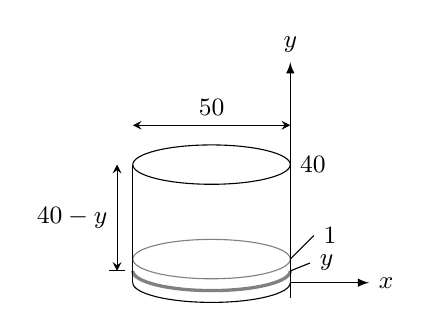
\begin{tikzpicture}[font=\small]
\pgfmathsetmacro{\h}{1.5}
\pgfmathsetmacro{\r}{1}
\pgfmathsetmacro{\t}{0.3}
\draw[-latex](\r,0)--++(1,0)node[right]{$x$};
\draw[-latex](\r,-0.2)--++(0,\h+1.5)node[above]{$y$};
\draw([shift={(180:\r cm and 1/4*\r cm)}]0,0) arc (180:360:\r cm and 1/4*\r cm);
\draw[very thick,gray]([shift={(180:\r cm and 1/4*\r cm)}]0,\t/2) arc (180:360:\r cm and 1/4*\r cm);
\draw[gray](0,\t) circle (\r cm and 1/4*\r cm);
\draw(0,\h) circle (\r cm and 1/4*\r cm);
\draw(-\r,0)--++(0,\h)  (\r,0)--++(0,\h);
\draw[stealth-stealth](-\r,\h+0.5)--++(2*\r,0)node[pos=0.5,above]{$\SI{50}{\meter}$};
\draw(\r,\t)--++(0.3,0.3)node[right]{$1$};
\draw(\r,\t/2)--++(0.25,0.1)node[right]{$y$};
\draw[stealth-stealth](-\r-0.2,\t/2)--(-\r-0.2,\h)node[pos=0.5,left]{$40-y$};
\draw(-\r-0.1,\t/2)--++(-0.2,0);
\draw(\r,\h)node[right]{$40$};
\end{tikzpicture}
\caption{بیلنی حوض برائے مثال \حوالہ{مثال_تکمل_استعمال_بیلنی_حوض_نچلی_پٹی_ٹھیک}}
\label{شکل_مثال_تکمل_استعمال_بیلنی_حوض_نچلی_پٹی_ٹھیک}
\end{minipage}
\end{figure}

\موٹا{قوت سیال کا حصول}\\
کسی بھی محددی نظام میں سیال میں ڈوبے ہوئے انتصابی تختی کی ایک طرف پر قوت سیال حاصل کرنے کے لئے درج ذیل اقدام کریں۔
\begin{enumerate}[a.]
\item
نمائندہ افقی پٹی کی لمبائی اور گہرائی کی عمومی کلیہ تلاش کریں۔
\item
انہیں آپس میں ضرب دے کر سیال کی کثافت اور ثقلی مستقل \عددی{g=\SI{9.8}{\meter\per\second^2}} سے ضرب دے کر تکمل کو موزوں حدود کے بیچ حل کریں۔ 
\end{enumerate}

\ابتدا{مثال}\شناخت{مثال_تکمل_استعمال_بیلنی_حوض_نچلی_پٹی_ٹھیک}
ہم اب مثال \حوالہ{مثال_تکمل_استعمال_بیلنی_حوض_نچلی_پٹی} میں بیلنی حوض کی نچلی ایک میٹر چوڑی پٹی پر قوت سیال کی بالکل ٹھیک قیمت معلوم کر سکتے ہیں۔

ہم حوض کی تلا کو \عددی{y=0} پر رکھتے ہیں  (شکل \حوالہ{شکل_مثال_تکمل_استعمال_بیلنی_حوض_نچلی_پٹی_ٹھیک}) جبکہ محدد \عددی{y} کو اوپر کے رخ رکھتے ہیں۔ ہم \عددی{y} پر نمائندہ افقی پٹی کے لئے درج ذیل لکھ سکتے ہیں۔
\begin{enumerate}[a.]
\item
گہرائی پٹی:\quad
$40-y$
\item
لمبائی پٹی:\quad
$50\pi$
\end{enumerate}
یوں ایک میٹر چوڑی پٹی پر قوت درج ذیل ہو گی۔
\begin{align*}
F&=\int_0^1 \rho g (\text{\RL{گہرائی}})(\text{\RL{لمبائی}})\dif y=\int_0^1 \rho g (40-y)(50\pi)\dif y\\
&=9800(50\pi)\int_0^1(40-y)\dif y=\SI{60805525.81}{\newton}
\end{align*}  
\انتہا{مثال}
%========================

اس مثال میں حاصل قوت مثال \حوالہ{مثال_تکمل_استعمال_بیلنی_حوض_نچلی_پٹی} سے  کچھ کم ہے جو متوقع تھا۔


\جزوحصہء{قوت سیال اور وسطانی مرکز}
